%%%%%%%%%%%%%%%%%%%%%%%%%%%%%%%%%%%%%%%%%
% Dictionary
% LaTeX Template
% Version 1.0 (20/12/14)
%
% This template has been downloaded from:
% http://www.LaTeXTemplates.com
%
% Original author:
% Vel (vel@latextemplates.com) inspired by a template by Marc Lavaud
%
% License:
% CC BY-NC-SA 3.0 (http://creativecommons.org/licenses/by-nc-sa/3.0/)
%
%%%%%%%%%%%%%%%%%%%%%%%%%%%%%%%%%%%%%%%%%

%----------------------------------------------------------------------------------------
%	PACKAGES AND OTHER DOCUMENT CONFIGURATIONS
%----------------------------------------------------------------------------------------

\documentclass[10pt,a4paper,twoside]{article} % 10pt font size, A4 paper and two-sided margins

\usepackage[top=3.5cm,bottom=3.5cm,left=3.7cm,right=4.7cm,columnsep=30pt]{geometry} % Document margins and spacings

\usepackage[utf8]{inputenc} % Required for inputting international characters
\usepackage[T1]{fontenc} % Output font encoding for international characters

\usepackage{palatino} % Use the Palatino font

\usepackage{microtype} % Improves spacing

\usepackage{multicol} % Required for splitting text into multiple columns

\usepackage[bf,sf,center]{titlesec} % Required for modifying section titles - bold, sans-serif, centered

\usepackage{fancyhdr} % Required for modifying headers and footers
\fancyhead[L]{\textsf{\rightmark}} % Top left header
\fancyhead[R]{\textsf{\leftmark}} % Top right header
\renewcommand{\headrulewidth}{1.4pt} % Rule under the header
\fancyfoot[C]{\textbf{\textsf{\thepage}}} % Bottom center footer
\renewcommand{\footrulewidth}{1.4pt} % Rule under the footer
\pagestyle{fancy} % Use the custom headers and footers throughout the document

\newcommand{\entry}[4]{\markboth{#1}{#1}\textbf{#1}\ {(#2)}\ \textit{#3}\ $\bullet$\ {#4}}  % Defines the command to print each word on the page, \markboth{}{} prints the first word on the page in the top left header and the last word in the top right

\usepackage{tikz}
\usetikzlibrary{calc} % Optional, but useful for more complex calculations


%----------------------------------------------------------------------------------------

\begin{document}

%----------------------------------------------------------------------------------------
%	TITLE PAGE
%----------------------------------------------------------------------------------------


\begin{titlepage}

\AddToHookNext{shipout/background}{
    \begin{tikzpicture}[remember picture, overlay]
        \node at ($(current page.south) + (0, 8.25cm)$) % Adjust 1cm for desired distance from bottom
            {\centering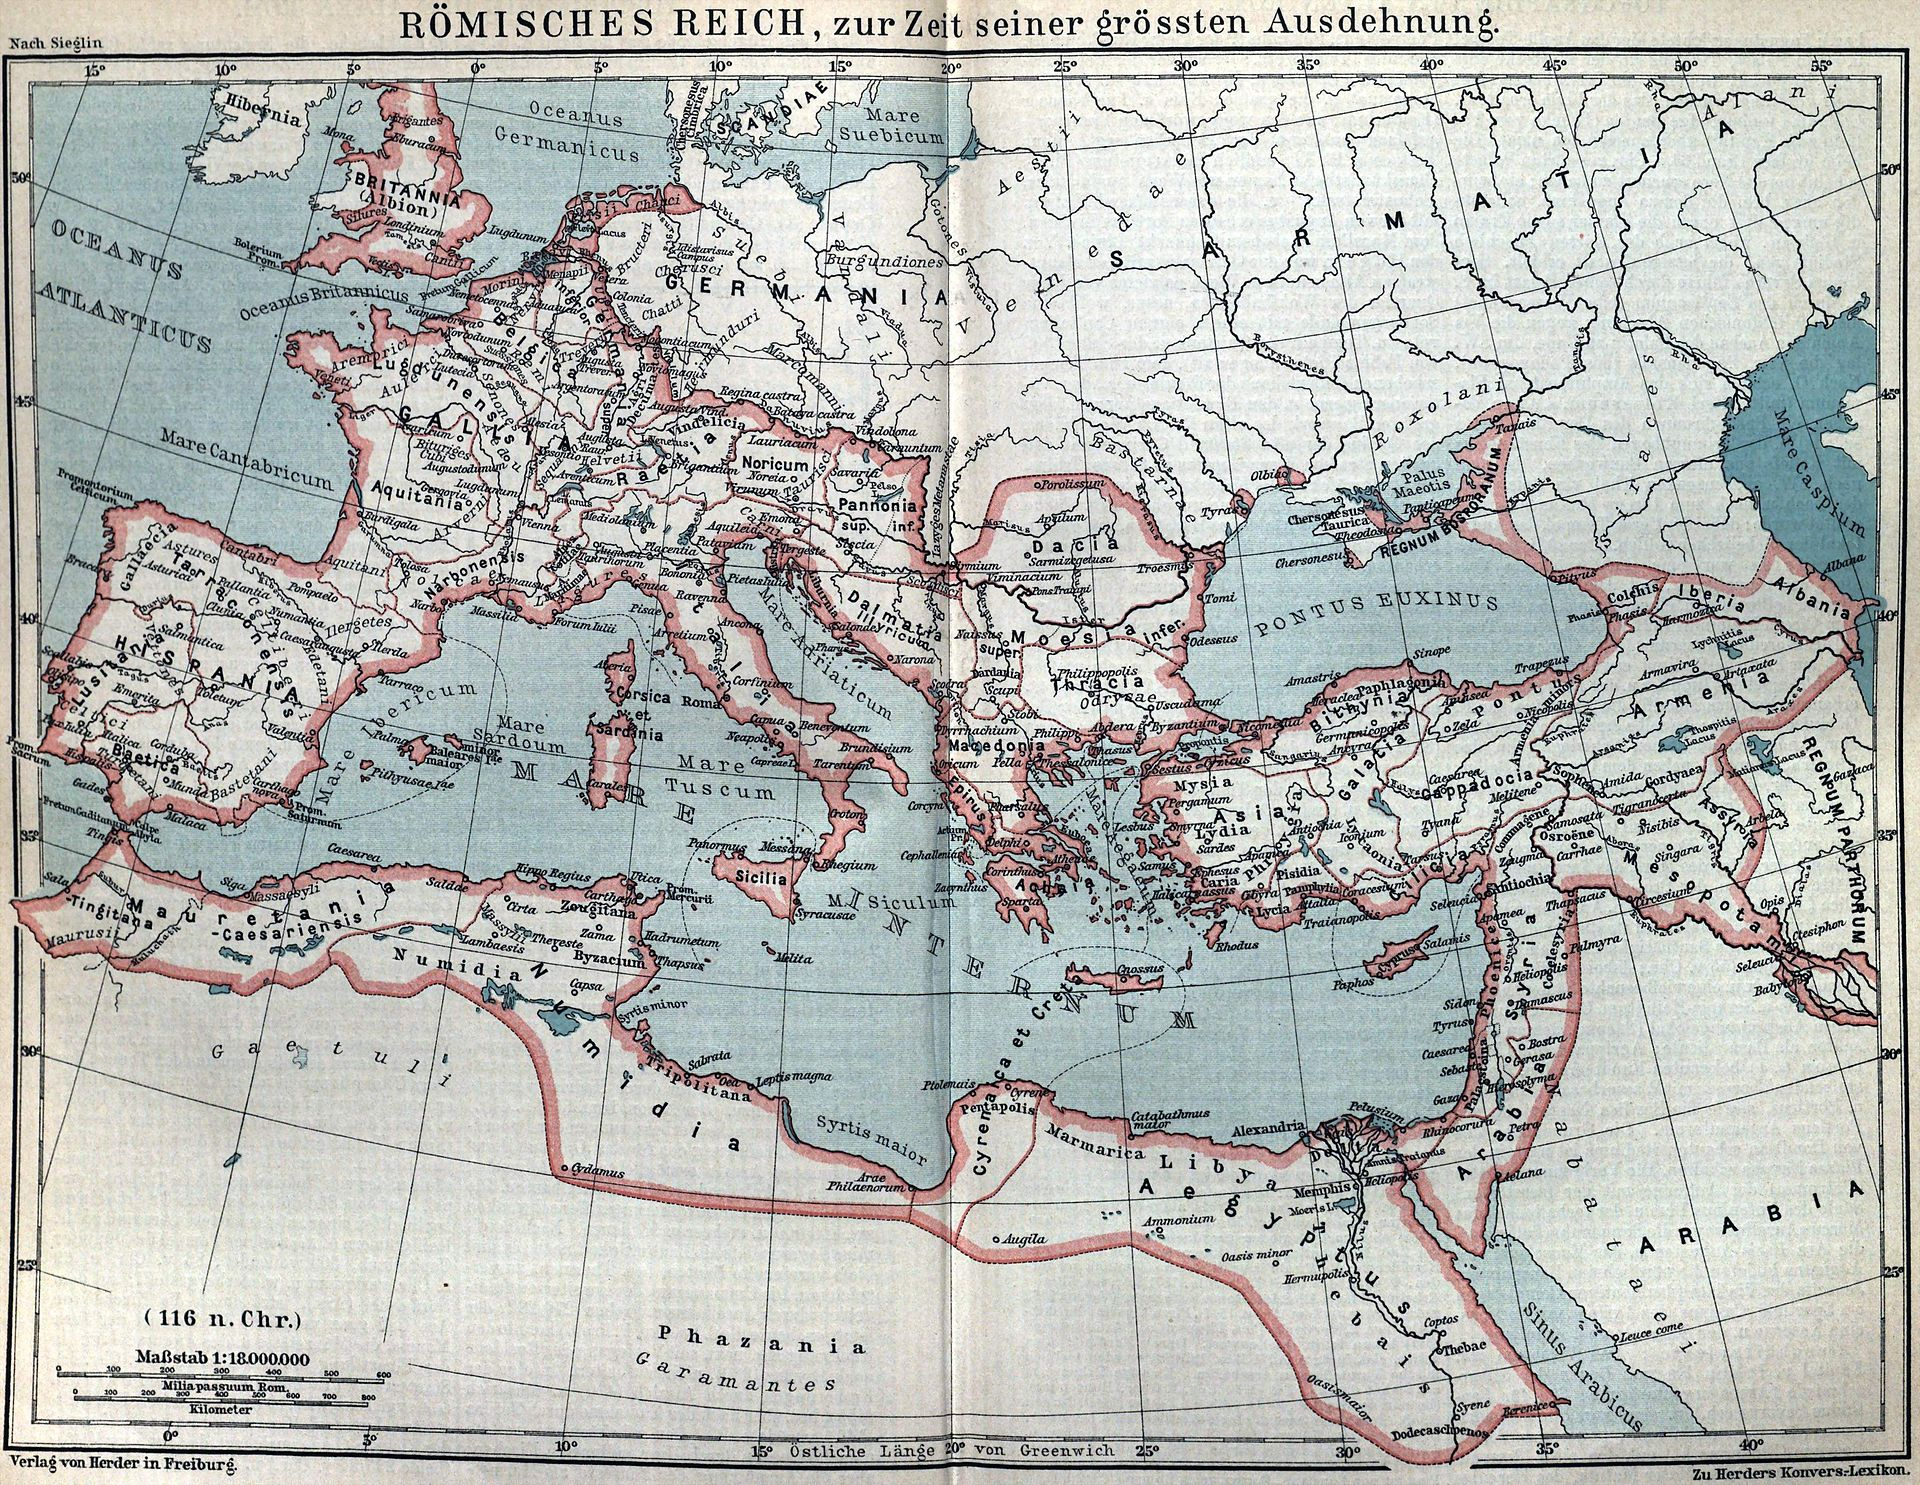
\includegraphics[width=1.5\textwidth]{Regnum_Bosporanum}}; % Adjust width and image filename
    \end{tikzpicture}
}


  \centering % Center all content
    \vspace*{2cm} % Add vertical space from the top
    {\Huge Xersonesus \\} % Large title
    \vspace{1cm}
    {\Large An Historical and Critical Encyclopedia of the Ukraine War \\} % Subtitle
    \vspace{2cm}
    {\Large 3AC3B33B33B53BB3BF3C2 \\} % Author name
    {\normalsize \emph{ seppie coi piselli alla romana } \\}
    \vspace{1cm}
    {\today} % Date
    \vfill % Fill remaining vertical space
    % Add any other elements like logos, disclaimers, etc.


 \end{titlepage}

%----------------------------------------------------------------------------------------
%	SECTION A
%----------------------------------------------------------------------------------------

\section*{A}

\begin{multicols}{2}

\entry{Artillery} {ar·til·ler·y} {Noun} {Coined by the gravedigger of the revolution, Joseph Stalin, artillery is the god of war. The god of war, however, is now but only a vital component in an evolving array of combined arms in eastern Europe.}



\end{multicols}

%----------------------------------------------------------------------------------------
%	SECTION B
%----------------------------------------------------------------------------------------

\section*{B}

\begin{multicols}{2}

\entry{Bombing} {bomb·ing} {Gerund} {Bombing has thus far been ineffective from the beginning of the Ukraine war. It alone has not accomplished a single strategic objective for any of the warring parties. 

}

\end{multicols}

%----------------------------------------------------------------------------------------
%	SECTION C
%----------------------------------------------------------------------------------------

\section*{C}

\begin{multicols}{2}

\entry{CIA} {Abbreviation} {Noun} {

It is often claimed in print that the CIA (Central Intelligence Agency) predicted the beginning of the Ukraine war. It is true. The CIA forecast Russia's full-scale invasion less than two weeks in advance. In the publications in Ukrainian, Hebrew, Russian, or English, the majority of the accompanying images are pulled directly from an article published seven years ahead of its time. On Mar 9, 2015, \emph{Stratfor} published its famous article, "Gaming a Russian Offensive." The scenarios the CIA discusses in its forecast are replications of those from \emph{Stratfor}'s article. The arrows in these sets of images follow those in \emph{Stratfor}'s article.  \newline \indent It is interesting how these new images spiral outward from a common source almost like a Fibonacci sequence, adding more arrows with the fractionalization of the original scenarios. 

}


\end{multicols}

%----------------------------------------------------------------------------------------
%	SECTION R
%----------------------------------------------------------------------------------------

\section*{R}

\begin{multicols}{2}

\entry{Russia} {Russ·ia} {Noun} {

Russia is one of the belligerents in the Ukraine war. 

}


\end{multicols}

%----------------------------------------------------------------------------------------
%	SECTION S
%----------------------------------------------------------------------------------------

\section*{R}

\begin{multicols}{2}

\entry{Shahed} {Sha·hed} {Noun} {

Russia launched its first Shahed, one of the most important evolving weapons in the Ukraine war, in the immediate aftermath of its defeat in the face of the great Ukrainian offensive in Kharkiv   launched on September 6th, 2022. \newline \indent Debate rages around the modifications, versions, or models of Shaheds involved in legendary attacks, which Russian or Iranian factory produced them, the country of origin responsible for, or the actual nature, underlying engineering, or specification of the most distinguished parts, components or kits.  

}

\entry{Syria} {Syr·ia} {Noun} {

The collapse of Syria's Assad regime, a fifty year old dynasty, is a result of the Ukraine war. 

}


\end{multicols}


%----------------------------------------------------------------------------------------
%	SECTION T
%----------------------------------------------------------------------------------------

\section*{R}

\begin{multicols}{2}

\entry{Time} {Ti·me} {Noun} {

It is to be determined which of the most prized possessions in warfare, time or space, the belligerents seek or exploit at any given phase of the Ukraine war. 

}


\end{multicols}

%------------------------------------------------
\end{document}